% Генетический алгоритм декомпозиции расчетной сетки.
\subsection{Генетический алгоритм декомпозиции неструктурированной расчетной сетки}\label{sec:text_2_genetic}

Генетические алгоритмы представляют собой природоподобные эвристические алгоритмы, с помощью которых можно искать решения оптимизационных задач с большим количеством параметров \cite{Chahar2021Gen,Wirayanti2025Gen}.
В процессе применения генетического алгоритма моделируется процесс создания, выживания и размножения популяции потенциально возможных решений поставленной проблемы в условиях сложно устроенной окружающей среды.
Применимость генетических алгоритмов базируется на принципе выживания сильнейших особей в популяции \cite{Naaman2025Gen}.
Работа генетического алгоритма начинается с создания стартовой популяции потенциальных решений проблемы, каждое решение представлено отдельной особью, а каждая особь определяется набором характеризующих ее генов (генотипом).
Для особи должна быть определена функция пригодности, которая является индикатором качества особи для решения поставленной задачи (вместо функции пригодности можно использовать штрафную функцию, которая наоборот является показателем непригодности). 

Генетический алгоритм является итерационным.
На каждой итерации по определенным законам на основе текущей популяции создается следующая популяция, которая по ожиданиям в среднем должна быть более приспособлена к условиям окружающей среды (то есть лучше удовлетворять решению поставленной задачи).
Процесс получения новых популяций продолжается до тех пор, пока не будет достигнуто некоторое условие (либо получено решение требуемого качества, либо дальнейшее улучшение не наблюдается) \cite{Charilogis2024Gen}.
Генетические алгоритмы широко применяются во многих областях, для решения задач с большим количеством параметров и ограничений.
Конечно, применение генетических алгоритмов не подразумевает отыскание оптимального решения, однако с их использованием можно быстро найти решение, которое является достаточно качественным в текущих условиях.
Генетические алгоритмы применимы для решения задач планирования \cite{Dawei2025Gen} и эффективного использования ресурсов \cite{Fang2025Gen,Mahmood2024Gen}.
Они используются для анализа данных, поиска тенденций и предсказаний, где не могут быть получены точные решения \cite{Kangra2024Gen,Sangeetha2025Gen}.
Одна из областей активного применения генетических алгоритмов – задачи комбинаторной оптимизации \cite{Hamdan2023Comb,Odeyemi2025Comb}.
При решении задач комбинаторной оптимизации точное решение зачастую не может быть получено из-за большого количества параметров и отсутствия полиномиального алгоритма для решения поставленной проблемы.
Генетические алгоритмы позволяют находить приемлемые решения для таких классических задач, как задача коммивояжера \cite{Kralev2024Gen}, задача нахождения оптимального пути \cite{Bogdanov2023Gen}, раскраска графа \cite{Malhotra2024Graph}, декомпозиция графа \cite{Chaouche2023Graph,Li2020Graph}.

При использовании генетических алгоритмов важно различать понятие генотипа и особи.
Генотип – это набор генов, некий код, который кодирует механизм создание особи.
Особь – сформированный на основе генотипа индивид, который обладает определенными свойствами и характеристиками, и для которого может быть вычислена функция пригодности или штрафная функция.
Зачастую при использовании генетических алгоритмов различие между генотипом и особью стирается, и вместо генотипа используется просто явное представление особи.
Так в работе \cite{Chaouche2023Graph} при декомпозиции графа в генотипе кодируется каждое ребро рассматриваемого графа, а в работе \cite{Li2020Graph} генотип представляет собой точное соотнесение каждой вершины графа и результирующего домена.
Использование генотипа в роли особи в генетических алгоритмах приводит к существенному замедлению сходимости, что снижает ценность использования этих алгоритмов.
К тому же применение механизмов скрещивания и мутаций к особям вместо генотипов также вызывает сомнение с точки зрения корректности таких операций. В данной работе предлагается подход, в котором в качестве генотипа используется максимально короткий код, по которому может быть быстро построена особь.

\subsubsection{Описание алгоритма}

Рассмотрим алгоритм декомпозиции дуального графа произвольной расчетной сетки на $k$ доменов.
Количество вершин в графе равно $n$.
При этом рассматриваемый дуальный граф задан структурами \texttt{inc} и \texttt{es}.
В структуре \texttt{inc} хранятся соседи каждой вершины графа: \texttt{inc[i]} -- вектор номеров всех вершин, смежных $i$-й вершине.
Структура \texttt{es} -- множество ребер графа.

В качестве особи будем рассматривать вектор \texttt{domains} длины $n$, в котором \texttt{domains[i]} -- номер домена, к которому отнесена $i$-ая вершина графа.
В качестве функции качества особи будем использовать функцию $Q = \delta D + \lambda L$ (чем ниже значение данной функции, тем выше качество особи) с весами $\delta = 10$ и $\lambda = 1$.
Исходя из этого, функцию $Q$ можно называть штрафной функцией особи.
Под популяцией будем понимать набор отдельных особей.

Ключевым элементом генетического алгоритма является понятие генотипа и процесс формирования особи на основе генотипа.
В качестве генотипа будем использовать вектор \texttt{genotype} длины $k$, задающий $k$ номеров вершин дуального графа, которые будем называть опорными вершинами.
При инициализации каждую опорную вершину \texttt{genotype[i]} будем принудительно относить к $i$-му домену.
При построении особи на основе генотипа будем распределять вершины между доменами с помощью простого алгоритма, схожего с алгоритмом пузырькового роста, начиная с опорных вершин и обходя граф в ширину.
Программный код процедуры распределения вершин между доменами можно видеть на листинге~\ref{lst:text_2_gen_alg}.

\begin{lstlisting}[caption={Простая декомпозиция, используемая в генетическом алгоритме.},label={lst:text_2_gen_alg}]
deque<size_t> q;

for (auto i { 0 }; i < k; ++i)
{
    domains[genotype[i]] = i;
    q.push_back(genotype[i]);
}

while (!q.empty())
{
    auto node { q.front() };
    auto domain { domains[node] };
    q.pop_front();

    for (auto ngh : inc[node])
    {
        if (domains[ngh] == -1)
        {
            domains[ngh] = domain;
            q.push_back(ngh);
        }
    }
}
\end{lstlisting}

Приведенный на листинге~\ref{lst:text_2_gen_alg} алгоритм декомпозиции по опорным вершинам не является сколь угодно оптимальным (и даже намеренно взят наиболее простым) и создает несбалансированные разбиения, зато он является быстрым, что позволяет создавать большое количество особей за короткое время.

На основе выбранного простого способа построения особи будем моделировать процесс эволюции следующим образом.
Пусть мы имеем текущую популяцию, в которой для каждой особи известна характеристика ее качества (эта характеристика вычисляется при построении особи и не меняется на протяжении всей ее жизни).
На первой фазе будем удалять некоторое количество наихудших особей из популяции.
Из оставшейся популяции случайно сформированные пары особей на основе операции скрещивания (кроссовера) будут производить потомство и добавлять в популяцию для восстановления ее исходного размера.
Операция скрещивания устроена предельно просто: для каждого номера $i$ от $1$ до $k$ в качестве $i$-го гена случайным образом выбирается $i$-й ген одного из родителей.
После выполнения скрещивания в новой особи с заданной вероятностью применяется мутация (см. рис.~\ref{fig:text_2_genetic_cross_mut}).

\begin{figure}[ht]
\centering
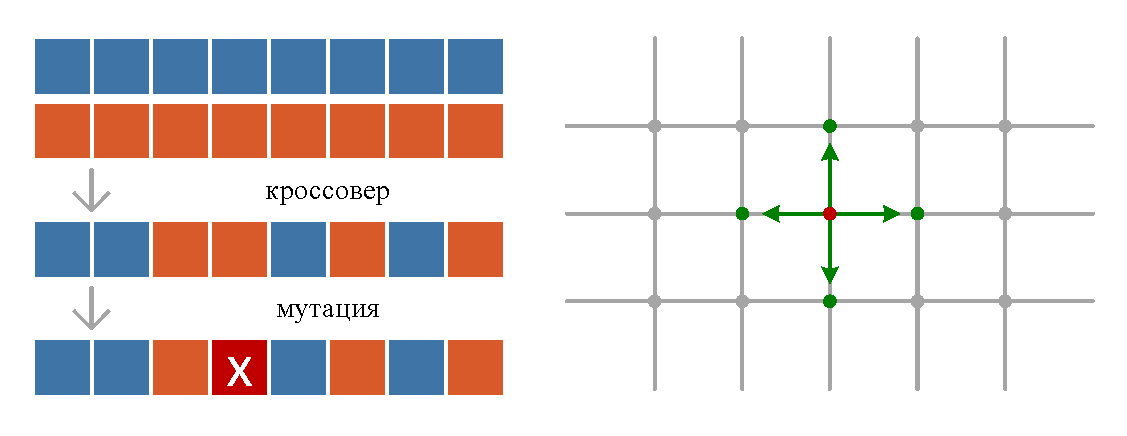
\includegraphics[width=0.8\textwidth]{./pics/text_2_genetic/cross-mut.pdf}
\singlespacing
\captionstyle{center}\caption{Схема кроссовера и мутации новой особи.}
\label{fig:text_2_genetic_cross_mut}
\end{figure}

Так как ген представляет собой номер опорной вершины дуального графа, то в качестве мутации выбрана операция замены случайной опорной вершины на выбранную случайным образом смежную с ней вершину (см. рис.~\ref{fig:text_2_genetic_cross_mut}, справа).

Описанный генетический алгоритм поиска эффективной декомпозиции характеризуется следующими глобальными параметрами. Количество эпох (\texttt{epochs\_count}) -- количество последовательных применяемых глобальных операций по вымиранию части популяции и ее восстановлению.
Размер популяции особей (\texttt{population\_size}) -- количество особей в популяции.
Доля вымирания (\texttt{extinction\_ratio}) – доля наименее эффективных особей, вымирающих на каждой эпохе.
Вероятность мутации (\texttt{mutation\_propability}) -- вероятность мутации в новой особи.

\subsubsection{Эксперимент по применению генетического алгоритма}

Будем применять описанный выше генетический алгоритм для решения задачи декомпозиции двумерной прямоугольной структурированной расчетной сетки размером $100 \times 100$ ячеек.
Такой вид сетки выбран для удобства визуализации результатов, сам алгоритм применим для расчетных сеток произвольного вида, так как на вход он принимает только информацию о структуре дуального графа.

Количество параметра \texttt{epochs\_count} выбрано равным 500.
Алгоритм прекращает работу либо после обработки последней эпохи, либо после того, как все особи в популяции сравняются по характеристике эффективности.

Размер популяции \texttt{population\_size} выбран равным 50.
При выборе размера популяции необходимо придерживаться баланса.
При слишком большом значении этого параметра время работы алгоритма существенно возрастает, а при слишком маленьком значении ограничивается разнообразие особей в популяции, что приводит к ранней остановке алгоритма в локальном минимуме, в котором все особи обладают одинаковым достаточно плохим показателем эффективности.

Доля вымирания \texttt{extinction\_ratio} принята равной 0,2.
При выборе доли вымирания не стоит использовать слишком высокие значения, так как это приводит к излишне интенсивному отсеву особей.
Это может привести к преждевременной отбраковке средних по эффективности особей, способных дать более эффективное потомство.

Вероятность возникновения мутации \texttt{mutation\_probability} принята равной 0,2.
Ввиду того, что мутация представляет собой смещение опорной вершины по ребру к одному из своих соседей (что является достаточно незначительным изменением), то такое частое возникновение мутаций оправдано.

\begin{figure}[ht]
\centering
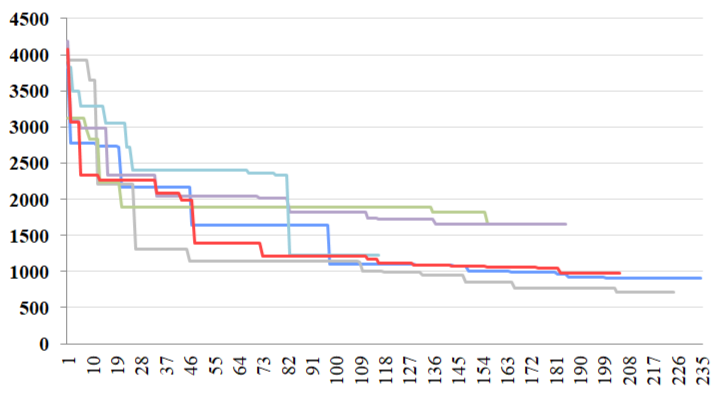
\includegraphics[width=0.8\textwidth]{./pics/text_2_genetic/chart1.png}
\singlespacing
\captionstyle{center}\caption{Характерные графики штрафной функции лучшей особи в популяции в зависимости от номера эпохи.}
\label{fig:text_2_genetic_chart1}
\end{figure}

Типичные графики значения штрафной функции лучшей особи в популяции от номера эпохи приведены на рис.~\ref{fig:text_2_genetic_chart1}.
Эксперименты показали, что при выбранном наборе макропараметров алгоритма примерно в первые 100 эпох наблюдается существенное улучшение лучшей особи в популяции, затем медленное улучшение наблюдается еще около 150 эпох, после чего работа алгоритма останавливается в локальном минимуме при заполнении всей популяции копиями лучшей особи.
При этом значение штрафной функции лучшей особи за время работы алгоритма падает примерно на 50-75\%, если считать от значения лучшей особи стартовой популяции.
Для повышения качества работы алгоритма можно включить механизм предотвращения его ранней остановки.
Для этого при возникновении копий лучшей особи можно применять к ней так называемые макромутации, что соответствует принудительному выталкиванию особи из локального минимума штрафной функции \cite{Baranov2025Gen}.

\begin{figure}[ht]
\centering
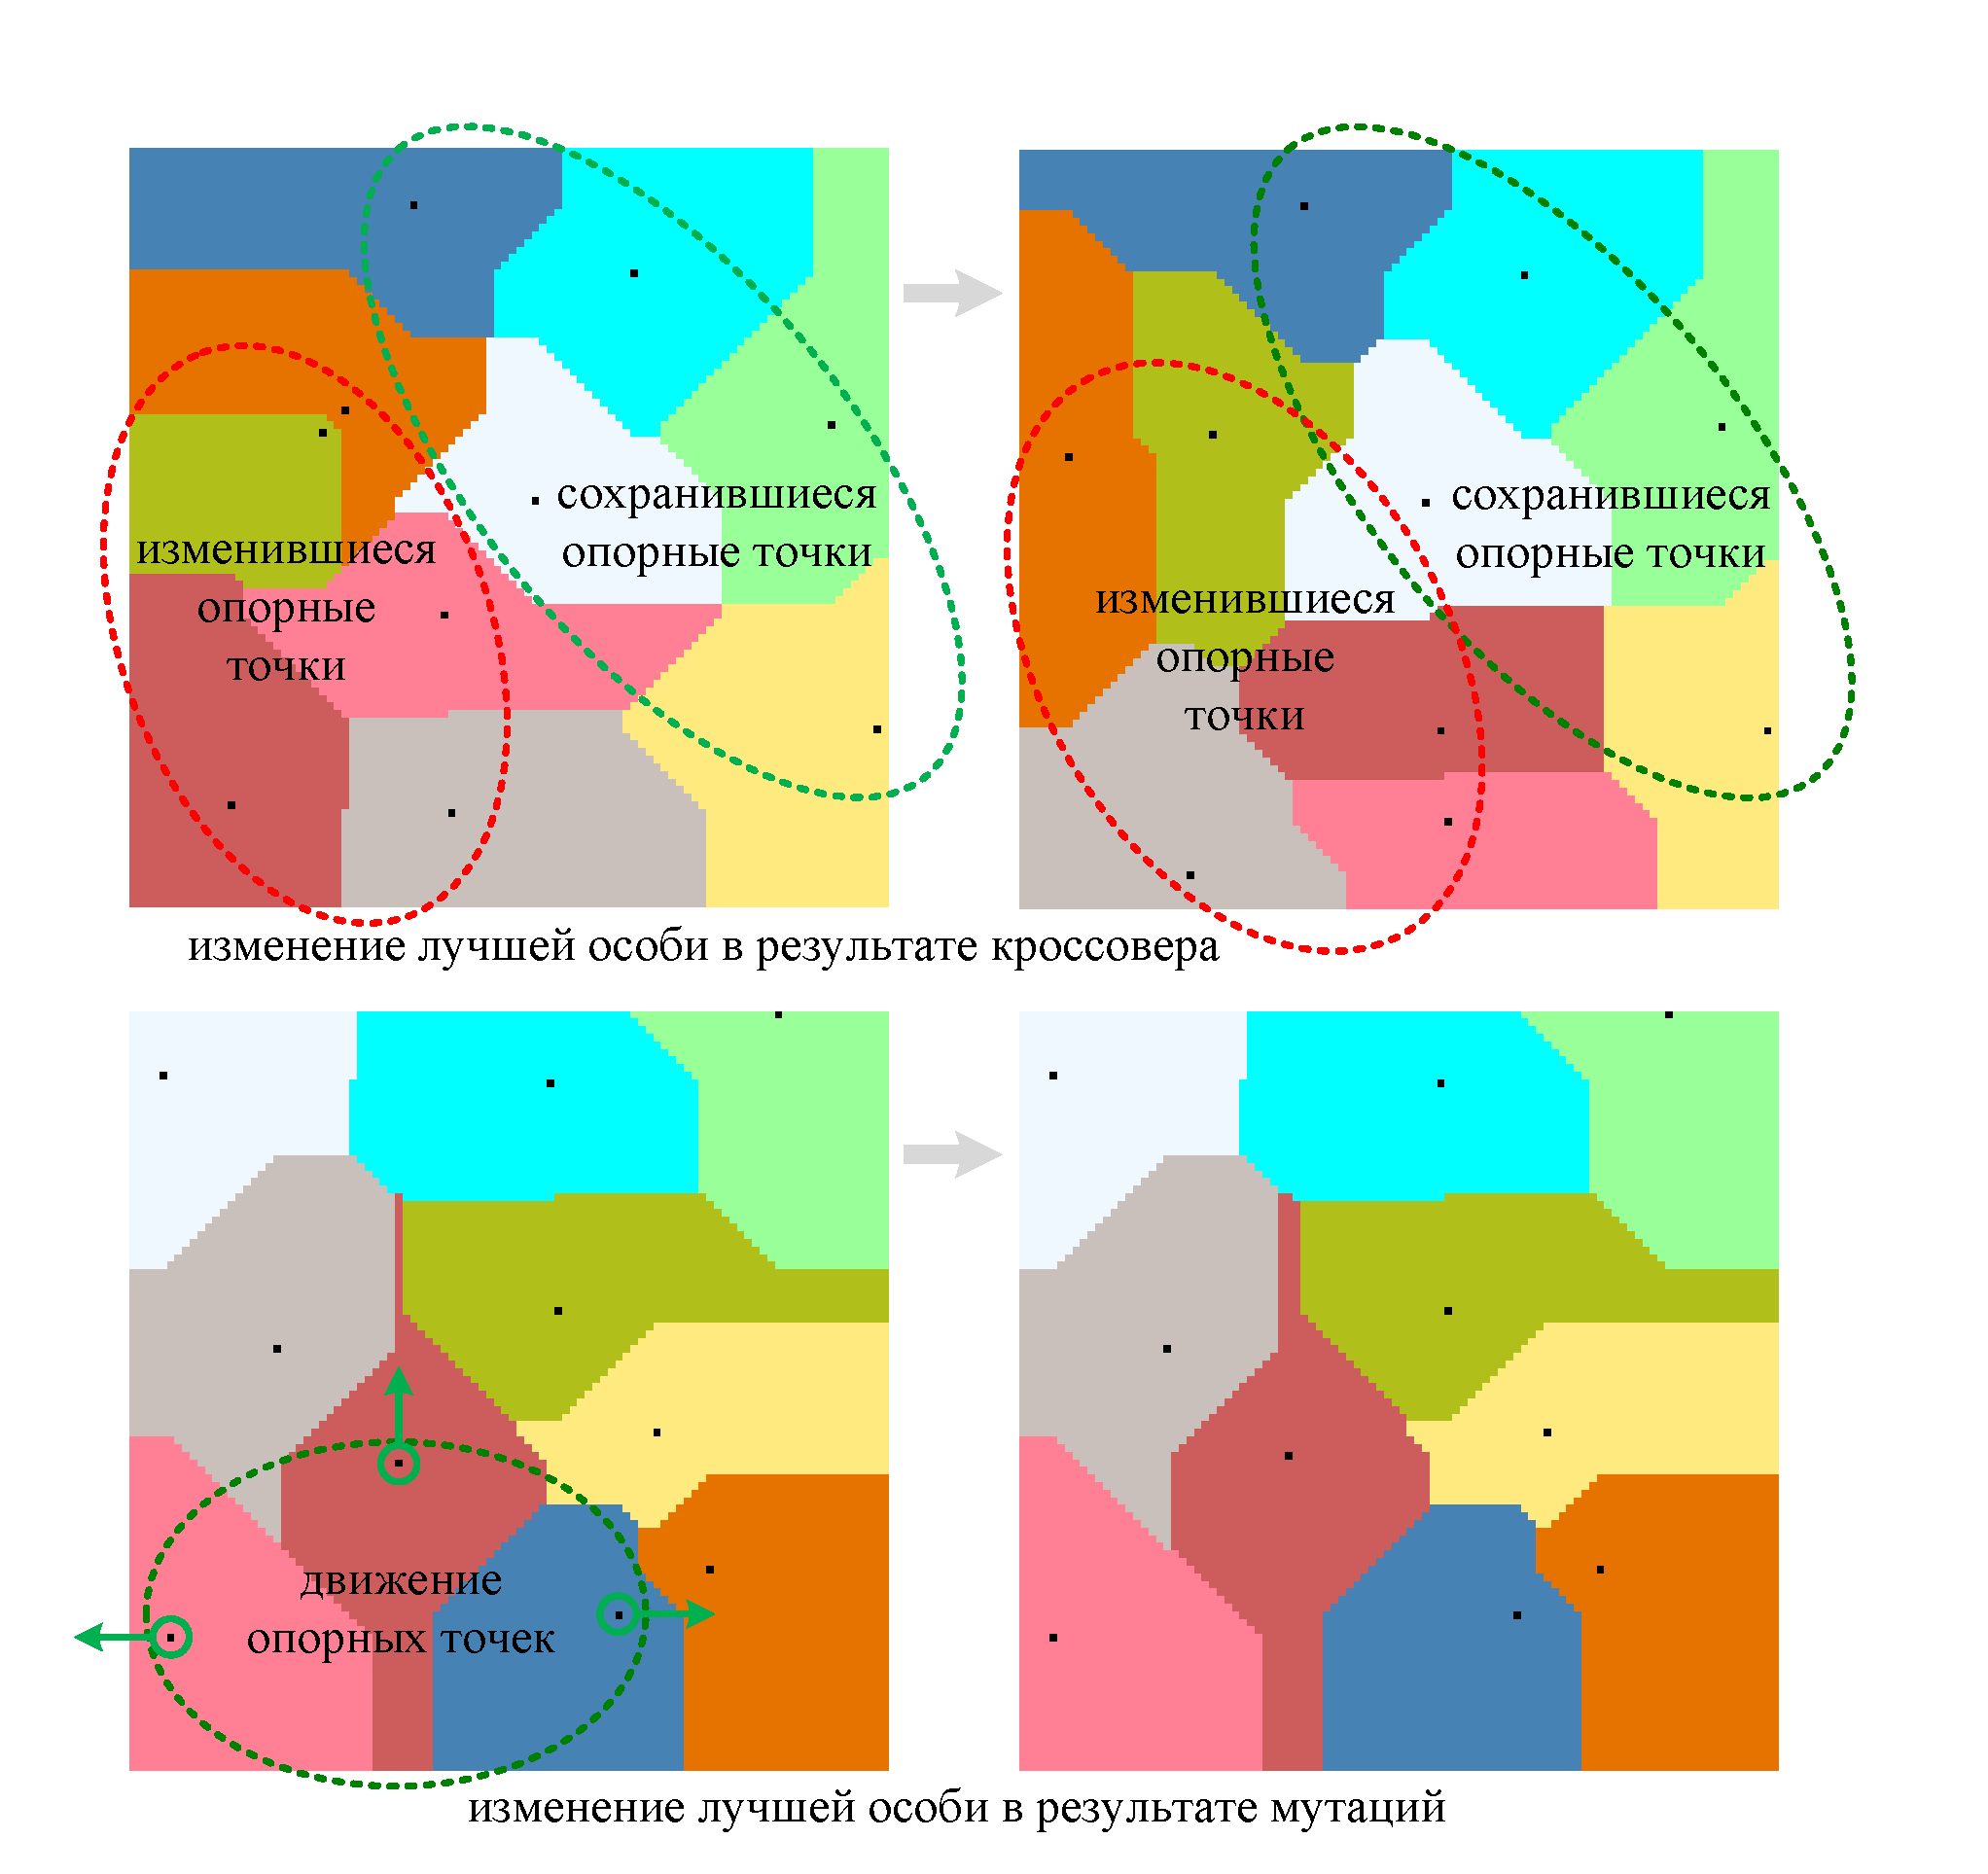
\includegraphics[width=0.8\textwidth]{./pics/text_2_genetic/changes.pdf}
\singlespacing
\captionstyle{center}\caption{Замещение части генотипа в процессе скрещивания (сверху), и мутация опорных вершин (снизу).}
\label{fig:text_2_genetic_changes}
\end{figure}

На рис.~\ref{fig:text_2_genetic_changes} приведены характерные варианты изменения лучшей особи при переходе от текущей популяции к популяции следующей эпохи.
Сверху на рисунке проиллюстрирована ситуация, когда часть опорных вершин лучшей особи сохранилась, а другая часть была заменена на опорные вершины второго родителя, что в целом привело к снижению значения штрафной функции.
Снизу на рисунке проиллюстрировано влияние последовательности мутаций на лучшую особь.
Так, даже незаметное на рисунке смещение опорных вершин привело к визуально различимому изменению геометрии образованных этими опорными вершинами доменов.

Следует отметить, что хоть реализация генетического алгоритма и подразумевает постоянное улучшение эволюционирующей популяции, это никак не гарантируется.
Более того, при скрещивании двух особей нет гарантии, что их потомство будет более приспособленным к поставленной задаче.
Также отсутствует гарантия, что применяемые мутации всегда приводят к более качественному решению.
Поэтому возникает вопрос -- не является ли сам факт появления удачных особей случайным событием, и не было бы более эффективным просто сгенерировать большое количество случайных особей, после чего выбрать из них лучшего представителя.
Для проверки этого предположения были проведены следующие эксперименты.
Пусть у нас имеется одиночный запуск генетического алгоритма с макропараметрами \texttt{population\_size} и \texttt{extinction\_ratio}.
Если в процессе работы алгоритма до его завершения прошло \texttt{ecount} эпох (не считая стартовой), то всего было создано \texttt{icount} = \texttt{population\_size} × (1 + \texttt{ecount} × \texttt{extinction\_ratio}) особей.
Поэтому после завершения каждого запуска генетического алгоритма его результат сравнивался со значением лучшей особи из случайной популяции размера \texttt{icount}.
Результаты такого сравнения приведены на рис.~\ref{fig:text_2_genetic_chart2}.
Красным цветом отмечен график качества лучшей особи в начале работы алгоритма, зеленым -- в конце.
Черным цветом отмечено значение лучшей особи случайной популяции размера \texttt{icount}.
Также на графиках отмечены линии средних значений для серии запусков генетического алгоритма.
Результаты расчетов показали, что лучшая особь популяции генетического алгоритма опережает лучшую особь случайной популяции примерно в 1,5 раза.

\begin{figure}[ht]
\centering
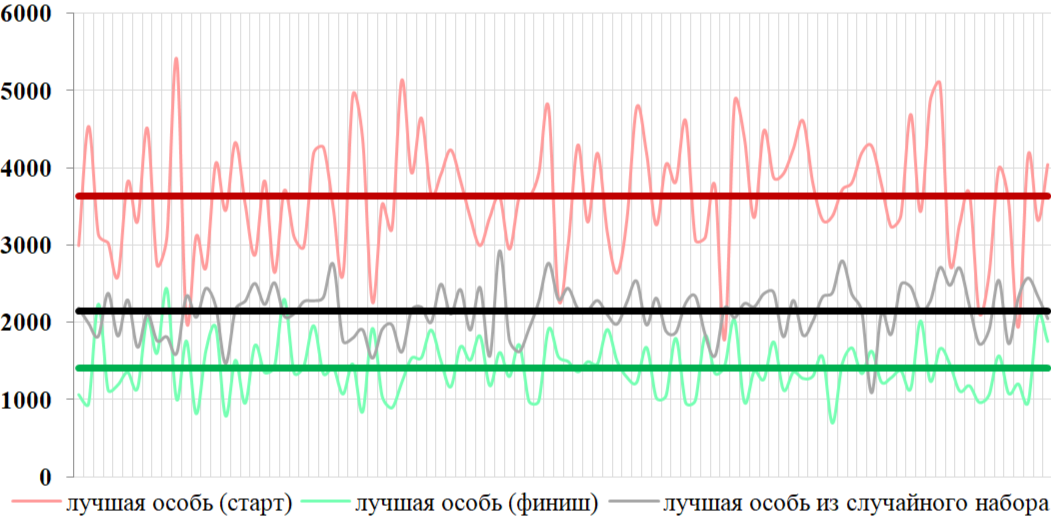
\includegraphics[width=0.8\textwidth]{./pics/text_2_genetic/chart2.png}
\singlespacing
\captionstyle{center}\caption{Сравнение лучшей особи в популяции генетического алгоритма с лучшей особью случайной популяции.}
\label{fig:text_2_genetic_chart2}
\end{figure}

Разработанный генетический алгоритм применим к расчетным сеткам произвольного вида, с его помощью можно быстро получать качественное решение декомпозиции, произвольным образом задавая требуемую штрафную функции решения.
Алгоритм допускает параллельное исполнение, хорошо масштабируется для работы с расчетными сетками большего размера.
Алгоритм может быть расширен с помощью других процедур генерации особи из генотипа.
